% AI-MD final report working draft, v5.
% Target: 9 pages in NeurIPS 2025 format.
% Source of truth for the systematic retrieval experiment and its downstream
% evaluation: commit 65335ab4a43f078deb42bca5c2ca791eca195a10.
% The earlier unsuccessful retrieval implementation is intentionally not treated
% as a separate research stage in this paper.

\documentclass{article}
% [final] = camera-ready: author names shown, no "preprint" banner, no line
% numbers. Removing the option entirely would switch neurips_2025 into
% anonymous submission mode (authors hidden, line numbers added), which would
% undo the named author block below, so [final] is the non-preprint form that
% keeps the authors visible.
\usepackage[final]{neurips_2025}
\usepackage[utf8]{inputenc}
\usepackage[T1]{fontenc}
\usepackage{hyperref}
\usepackage{url}
\usepackage{booktabs}
\usepackage{amsmath,amssymb,amsfonts}
\usepackage{nicefrac}
\usepackage{microtype}
\usepackage{xcolor}
\usepackage{graphicx}
\usepackage{tabularx}
\usepackage{array}
\usepackage{multirow}
\usepackage{placeins}
\usepackage{adjustbox}  % max width=\textwidth: shrink a wide table to fit, never enlarge

% Figures are generated by src/evaluation/presentation/final_report_figs.py and
% written to final_report/figures/ as vector PDF at \textwidth. The first path
% works when compiling inside final_report/, the second from the repository root.
\graphicspath{{figures/}{final_report/figures/}}
\newcommand{\best}[1]{\textbf{#1}}
\newcolumntype{Y}{>{\raggedright\arraybackslash}X}

% Float placement. This is a single-column format, so every float here is an
% ordinary figure/table, not a starred one: starred floats go through LaTeX's
% double-column output routine, which refuses 'h'/'b' and can never place a
% float on the page where it is declared, so all seven would be deferred and
% would land mid-paragraph. The defaults below are also too strict for seven
% large floats in nine pages -- textfraction 0.2 forbids any page from being
% more than 80% float, which forces the remaining text to be split awkwardly.
\renewcommand{\topfraction}{0.9}       % up to 90% of a page may be top floats
\renewcommand{\bottomfraction}{0.7}
\renewcommand{\textfraction}{0.07}     % allow float-heavy pages
\renewcommand{\floatpagefraction}{0.7} % a float page must be 70% full
\setcounter{topnumber}{3}
\setcounter{totalnumber}{4}

% Stop the large blank gaps between a float's caption and the text that resumes
% after it. Under \flushbottom, a page carrying a tall float plus a long caption
% has only a few lines of text left, and LaTeX makes the page bottom flush by
% inflating the glue above those lines -- which reads as the float having been
% torn away from the paragraph. \raggedbottom puts that slack at the foot of the
% page instead, where it is invisible, and the fixed separations below stop the
% remaining glue from stretching.
\raggedbottom
\setlength{\textfloatsep}{16pt plus 2pt minus 4pt} % float <-> text, top/bottom
\setlength{\floatsep}{14pt plus 2pt minus 3pt}     % float <-> float
\setlength{\intextsep}{14pt plus 2pt minus 3pt}

\title{Evidence Selection and Severity Reasoning for PHQ-8 Item-Level Prediction from Mental-Health Interviews}

\author{%
  Daniel Schmidt
  \And
  Yaniv Pevzner
}

\begin{document}
\maketitle

\begin{abstract}
Most automated depression-assessment systems predict a binary diagnosis or a single questionnaire total, obscuring the symptom profile that produced that score. We study the harder task of predicting each of the eight PHQ-8 item severities, on an ordinal scale from 0 to 3, from E-DAIC interview transcripts. The processed dataset contains 219 participants and 1,752 participant--item examples. We decompose the task into selecting item-relevant evidence from a long interview and inferring ordinal severity from that evidence. An initial participant-local hybrid retriever feeds a MentalBERT+CORN encoder and a Qwen2.5-7B reasoning model. The encoder produces fewer large ordinal errors but substantially under-detects severe symptoms; the LLM recovers more severe cases but makes more unsupported extreme predictions. Their complementary errors enable a selective Attention-MIL cascade, which remains the project-best system at macro-F1 0.409, QWK 0.447, and MAE 0.606. We then conduct a systematic, label-free retrieval experiment that separately tests audited Core, Lay, and Clinical vocabularies; natural-language semantic multi-queries; BM25 and semantic retrieval; hybrid weights; and evidence budgets. Lexicon expansion does not improve judged evidence quality. The selected retrieval configuration uses the Core vocabulary, 25\% BM25 and 75\% semantic scoring, and three windows, reaching an informative-evidence rate of 0.327. However, this retrieval improvement does not translate into a superior final predictor. Aggressively dropping judged-none training rows improves severe recall but also significantly increases false-severe predictions and removes most training examples. Leakage-safe cascades reduce ordinal error but do not surpass the frozen R0 cascade. These results show that evidence selection, severity reasoning, and safe model routing are related but distinct bottlenecks.
\end{abstract}

\section{Introduction}
\label{sec:introduction}
The Patient Health Questionnaire-8 (PHQ-8) assigns a frequency score from 0 to 3 to eight depressive symptoms and sums the items to a total from 0 to 24 \cite{kroenke2009phq8}. Although the total provides a compact severity measure, identical totals may arise from different symptom profiles. One participant may primarily report sleep and energy difficulties, whereas another may report depressed mood, anhedonia, and feelings of failure. Predicting the item profile can therefore preserve clinically meaningful structure that is lost when only an aggregate score is estimated.

Predicting item scores from a semi-structured interview is harder than completing the questionnaire directly. Evidence may be brief, indirect, distributed across the conversation, or absent from the transcript even when the participant endorsed the questionnaire item. We therefore formulate the problem as two coupled tasks. First, a retrieval mechanism must select transcript regions relevant to one PHQ-8 item. Second, an inference mechanism must map the selected evidence to an ordinal severity. Better retrieval need not yield better prediction: additional windows may add noise, and an expressive reasoning model may infer a symptom from general distress rather than item-specific evidence.

We investigate this decomposition using participant-local retrieval, an ordinal MentalBERT encoder, and an instruction-tuned LLM; Figure~\ref{fig:pipeline} summarizes the resulting study design. Controlled comparisons hold the evidence fixed to isolate severity reasoning. We then test whether the encoder and LLM can be combined selectively, and conduct a systematic retrieval experiment that separates vocabulary design, lexical and semantic matching, fusion weights, and evidence budget. All principal comparisons use participant-grouped out-of-fold (OOF) evaluation. Retrieved text is treated as candidate evidence, not as a validated clinical rationale.

Our contributions are fourfold. First, we formulate PHQ-8 prediction as 1,752 participant--item ordinal decisions with leakage-safe participant grouping. Second, we compare an ordinal encoder and explicit LLM reasoning on matched evidence, revealing a severe-sensitivity versus ordinal-safety trade-off. Third, we exploit their complementary errors through selective correction. Fourth, we perform a label-free retrieval study showing that audited Core queries, natural-language semantic multi-query retrieval, a light lexical contribution, and a small evidence budget are preferable to vocabulary expansion, while also demonstrating that better judged evidence does not automatically improve downstream prediction.

\section{Background and Related Work}
\label{sec:background}
DAIC-WOZ and E-DAIC provide semi-structured interviews and depression-related labels for computational mental-health research \cite{gratch2014daic,devault2014simsensei,ringeval2019avec}. Most prior systems predict depression status or an aggregate PHQ score, often using multimodal audio, visual, and linguistic signals. Our target differs: each PHQ-8 item is predicted separately from text, preserving an eight-dimensional symptom profile.

The closest formulations are question-wise or symptom-level models. QuestMF predicts question-level PHQ-8 scores through modality-specific fusion and an ordinal objective \cite{mandal2025questmf}. Milintsevich et al. estimate individual depressive symptoms from interview text, showing that symptom prediction can provide a more interpretable representation than total-score regression \cite{milintsevich2023symptom}. LMIQ prompts an LLM to complete psychiatric questionnaires from interviews and uses the structured responses for downstream prediction \cite{rosenman2024lmiq}. Our work instead retrieves participant-local evidence for each item, trains an ordinal item classifier, and compares its inference behavior with an LLM on matched evidence.

The retrieval and prediction components draw on established methods. BM25 provides sparse lexical matching \cite{robertson2009probabilistic}, whereas Sentence-BERT-style embeddings support semantic matching of paraphrases \cite{reimers2019sentencebert}. BERT provides the supervised encoder foundation \cite{devlin2019bert}, and MentalBERT adapts language models to mental-health text \cite{ji2022mentalbert}. Because item labels are ordered, we use CORN, which models conditional threshold decisions while enforcing rank-consistent probabilities \cite{shi2021corn,cao2020coral}. For LLM inference, chain-of-thought prompting and self-consistency motivate explicit severity reasoning and repeated sampled paths \cite{wei2022cot,wang2022selfconsistency}; Qwen2.5-7B-Instruct was selected as a locally runnable open-weight instruction model rather than through an exhaustive model benchmark \cite{qwen2025technical}.

\section{Methods}
\label{sec:methods}

\subsection{Task, Data, and Evaluation Protocol}
\label{subsec:data-eval}
For participant $i$ and PHQ-8 item $j$, the prediction task is
\begin{equation}
  f(U_i,q_j) \rightarrow \hat{y}_{ij}, \qquad y_{ij}\in\{0,1,2,3\},
\end{equation}
where $U_i$ is the interview transcript and $q_j$ is the item wording. The processed dataset contains 219 participants and eight rows per participant, yielding 1,752 participant--item examples. Label counts for classes 0, 1, 2, and 3 are 852, 513, 220, and 167, respectively.

Preprocessing normalizes identifiers and text, removes common non-verbal markers, validates item labels, and rejects duplicate participant--item keys. Context windows never mix participants. When reliable speaker fields are available, clear interviewer rows are excluded; otherwise the pipeline uses the available transcript lines. Because speaker roles are not uniformly reliable, retrieved excerpts are described as candidate evidence rather than verified question--answer rationales.

We use five-fold \texttt{StratifiedGroupKFold} with shuffling and seed 42, grouped by participant. All eight rows from a participant remain in one fold, and concatenated OOF predictions cover all 1,752 examples. Macro-F1 is the class-balanced headline metric; quadratic weighted kappa (QWK) measures ordinal agreement; and mean absolute error (MAE) measures severity distance. We additionally report class-3 F1, severe recall $P(\hat y=3\mid y=3)$, false-severe rate $P(\hat y=3\mid y<3)$, far-off error $P(|y-\hat y|\geq2)$, and accuracy within one level. Paired confidence intervals use 2,000 bootstrap resamples of whole participants, preserving the eight correlated rows contributed by each participant.

\subsection{Item-Conditioned Evidence Retrieval}
\label{subsec:retrieval}
\paragraph{Initial retrieval system.}
Each transcript is represented by participant-local context windows. Initial experiments compare single utterances with centered three- and five-turn windows (W3 and W5). BM25 ranks windows using the PHQ item text and a compact item glossary. A dense retriever encodes the item query and windows with \texttt{sentence-transformers/all-MiniLM-L6-v2}; normalized embeddings are compared by cosine similarity. The hybrid retriever merges candidates from the two modalities, assigns zero to a missing modality score, and min--max normalizes each score within the participant--item candidate set. Its score is
\begin{equation}
 s_{\mathrm{hyb}}(w)=\alpha\,\widetilde{s}_{\mathrm{BM25}}(w)
 +(1-\alpha)\,\widetilde{s}_{\mathrm{sem}}(w).
\end{equation}
The frozen Hybrid-W3 comparison uses $\alpha=0.5$, five selected windows, a candidate multiplier of five, and a maximum pairwise turn-overlap ratio of 0.5. The highest-ranked non-redundant windows are concatenated as evidence.

\paragraph{Systematic retrieval experiment.}
The systematic experiment holds the W3 window bank and participant folds fixed while independently varying three factors: query vocabulary, retrieval modality, and evidence budget. Four vocabulary configurations are evaluated: L0 Core; L1 Core+Lay; L2 Core+Clinical; and L3 Full. The clinical tier undergoes a provenance audit against standard symptom constructs and terminology: 146 candidates are reviewed, 101 retained, and 45 removed. The query artifacts are global and fold-independent; no transcript, label, or prediction is used to design them.

Semantic retrieval uses short natural-language queries rather than a concatenated keyword list. Each item has an item-meaning query, with optional Lay and audited Clinical queries according to the active vocabulary configuration. Sleep, Appetite, and Moving are represented with separate queries for their opposing poles. For a window $w$, semantic relevance is the maximum cosine similarity across active queries,
\begin{equation}
 s_{\mathrm{sem}}(w)=\max_{m\in\mathcal{Q}_j}
 \cos\bigl(e(q_{jm}),e(w)\bigr),
\end{equation}
so a strong match to one valid pole is not diluted by unrelated queries.

For every participant--item pair and vocabulary configuration, BM25-only and semantic-only systems rank the frozen W3 bank and retain Top-20 candidates after the same overlap-diversity rule. Per-window judgments cover the Top-10 unique candidates; set-level judgments evaluate Top-3, Top-5, and a MentalBERT token-budget prefix. BM25--semantic fusion is tested only after the single retrievers show two-sided complementarity. Hybrid weights are $\alpha\in\{0.25,0.50,0.75\}$, where $\alpha$ is the BM25 weight; thus $\alpha=0.25$ assigns 75\% of the fused score to semantic similarity.

The final retrieval configuration is selected without PHQ labels. The primary criterion is the set informative rate,
\begin{equation}
 P(\texttt{status}\in\{\texttt{supports},\texttt{against}\}).
\end{equation}
Candidates within 0.005 of the maximum are treated as tied; ties are broken by lower \texttt{none} rate, lower \texttt{ambiguous} rate, lower turn overlap, fewer windows, and finally the simpler retriever.

\subsection{Evidence-Quality Assessment}
\label{subsec:judge}
The evidence judge receives only an item and the retrieved text, never the gold PHQ label. It returns one of four statuses: \texttt{supports}, when the participant reports the symptom; \texttt{against}, when the participant clearly denies it or describes the opposite; \texttt{ambiguous}, when the text concerns the item but is insufficient or mixed; and \texttt{none}, when the text is not about the item. It may also return a severity hint only when frequency is explicit.

The final judge is Qwen2.5-7B-Instruct with three sampled completions at temperature 0.4, top-$p=0.9$, and a 96-token generation limit. Majority vote determines status; ties become \texttt{ambiguous}, and the median severity hint is used among chains supporting the winning status. An attempted substitution of locally available MentaLLaMA models failed validation because the models produced degenerate or valence-inverted judgments. Consequently, the judge and PHQ predictor belong to the same model family. All judge-derived retrieval and missing-evidence results are therefore model-based evidence audits, not clinician-validated evidence labels.

\subsection{Ordinal Encoder and Missing-Evidence Policies}
\label{subsec:encoder}
The encoder receives item text and retrieved evidence as a paired sequence separated by special tokens. The main backbone is \path{mental/mental-bert-base-uncased}. Matched experiments use AdamW, learning rate $2\times10^{-5}$, batch size 16, eight epochs, maximum length 256, and seed 42. BERT and MentalBERT backbones, cross-entropy variants, and ordinal losses are compared while holding the remaining configuration fixed.

For four severity classes, CORN learns three conditional binary decisions. If $z_k$ is the logit for threshold $k$, then
\begin{equation}
 P(y>k)=\prod_{r=0}^{k}\sigma(z_r).
\end{equation}
Class probabilities are obtained from adjacent cumulative differences, and the prediction is the number of cumulative threshold probabilities above 0.5. We also evaluate an Attention-MIL encoder that represents windows separately and aggregates them with learned gated attention; it later serves as a correction expert.

For the selected systematic retrieval, we compare three training policies. \emph{Status quo} retains every training row and its original gold label. \emph{Mask none} keeps judged-none rows in the batch but assigns them zero loss and excludes them from class-weight computation. \emph{Drop none} removes judged-none rows from both training and class-weight estimation. Validation rows are never removed or masked.

\subsection{LLM Severity Reasoning and Evidence Policies}
\label{subsec:llm}
The controlled per-item experiment uses \texttt{Qwen/Qwen2.5-7B-Instruct} in bfloat16 with the same Hybrid-W3 evidence as the frozen encoder. The prompt defines the four PHQ-8 frequency anchors and instructs the model to identify item-relevant excerpts, assess whether the symptom is absent, occasional, frequent, or persistent, and map the evidence to the nearest anchor without inventing unsupported symptoms. Four synthetic demonstrations, one per severity level, are included. Output is a JSON object containing a short rationale and label. Sampled self-consistency uses temperature 0.7, top-$p=0.9$, and majority voting.

We additionally evaluate cross-item reasoning. The \emph{Joint} prompt forms an overall impression and predicts all eight items in one pass. The \emph{Staged} prompt first scores items with clear evidence, constructs context only from confident items, and then resolves difficult items. The final tolerance-aware staged prompt prioritizes avoiding errors of at least two levels and reserves extreme labels for clear evidence. Five sampled chains yield item vote distributions and a \texttt{difficult\_frac}; two independent SC$\times$5 runs are pooled into a 10-chain prediction for the frozen LLM parent.

On the selected systematic retrieval, five inference policies are compared without changing model weights: keep the retrieved windows; filter per-window \texttt{none}; place \texttt{supports}/\texttt{against} before \texttt{ambiguous} and exclude \texttt{none}; fall back to a long transcript context when the selected set is \texttt{none} or filtering empties it; and use long context for every item as a retrieval-free control.

\subsection{Selective Correction}
\label{subsec:cascade}
The frozen R0 cascade is LLM-first. Confident LLM labels are retained; routed items are restricted to the LLM's two most probable classes, and an encoder chooses between those classes. The merged gate routes when either the largest LLM vote fraction is below 0.8 or \texttt{difficult\_frac}$\geq0.5$. It routes 41.5\% of examples. Attention-MIL provides the strongest correction branch.

For the final systematic retrieval, we evaluate new encoder-first and LLM-first cascades. Routing thresholds and item subsets are fitted inside each training fold rather than on OOF predictions. A cascade is accepted only if it improves over the better selected component without violating the predefined error and severe-class constraints.

\begin{figure}[tbp]
  \centering
  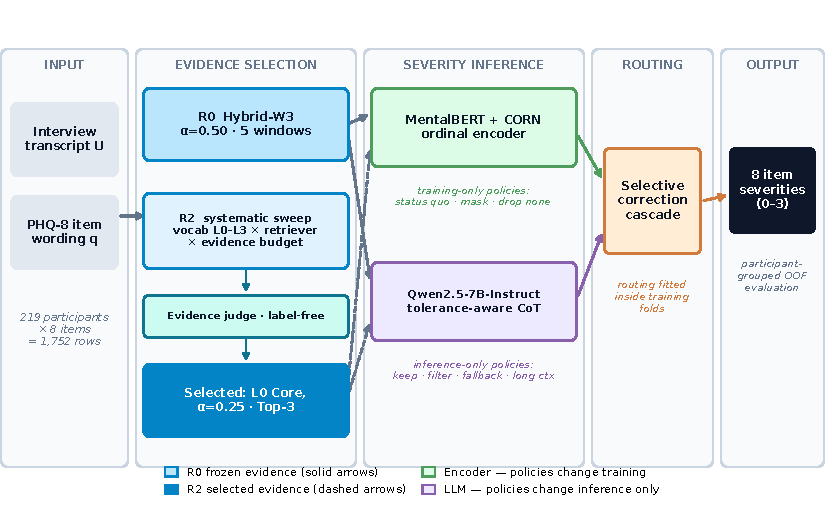
\includegraphics[width=\textwidth]{final_report_fig1_pipeline.pdf}
  \caption{End-to-end study design. Retrieval, evidence assessment, severity inference, and selective routing are evaluated as distinct components. Two evidence conditions feed the same two inference mechanisms: the frozen R0 Hybrid-W3 selector (solid arrows) and the R2 selector chosen by the label-free systematic sweep (dashed arrows). The evidence policies act at different points in the system. Encoder policies---status quo, mask none, and drop none---change the \emph{training} population and therefore require retraining, whereas LLM policies---keep, filter, informative-first, transcript fallback, and long context---change only the inference-time context and leave model weights untouched. The evidence judge scores retrieved sets without access to PHQ labels, so the retrieval configuration is selected label-free. All comparisons use participant-grouped out-of-fold evaluation over 219 participants and 1,752 participant--item rows.}
  \label{fig:pipeline}
\end{figure}

\section{Results}
\label{sec:results}

\subsection{Initial Retrieval, Severity Reasoning, and the Frozen Cascade}
\label{subsec:r0-results}
Table~\ref{tab:r0} reports the initial results. Context windows improve over a single retrieved utterance, and hybrid evidence improves ordinal agreement. MentalBERT with Hybrid-W5 and CORN is the strongest standalone encoder in the initial sweep, with macro-F1 0.372, QWK 0.390, and MAE 0.664. Hybrid-W3 is frozen for the controlled reasoning experiments because it provides a common evidence condition for the encoder and LLM.

The Hybrid-W3 MentalBERT+CORN encoder is exactly correct on 45.5\% of examples and within one level on 88.1\%. Its class-wise F1 nevertheless falls to 0.159 for class 3, and severe recall is only 0.102. Replacing only the inference mechanism with per-item CoT increases class-3 F1 to 0.295, but QWK falls and far-off error rises. Thus, the encoder is ordinally conservative, whereas the LLM is more severe-sensitive but less safe.

Unrestricted Joint reasoning performs worse than the final item-wise approach (macro-F1 0.339, QWK 0.334, MAE 0.727), consistent with a clinical-halo failure mode. Staged reasoning reduces this effect (0.355, 0.352, 0.686) but becomes too conservative for class 3. Pooled tolerance-aware self-consistency provides a stronger LLM parent at macro-F1 0.400, QWK 0.406, and MAE 0.641. The frozen Attention-MIL merged-gate cascade exploits encoder--LLM disagreement and remains the strongest complete system, at macro-F1 0.409, QWK 0.447, and MAE 0.606.

\begin{table}[tb]
  \caption{Initial participant-grouped OOF results. Panel A establishes the retrieval-conditioned ordinal baseline; Panel B compares severity reasoning and selective correction on frozen Hybrid-W3 evidence.}
  \label{tab:r0}
  \centering
  \scriptsize
  \adjustbox{max width=\textwidth}{%
  \begin{tabular}{lllrrrrr}
    \toprule
    Panel & Configuration & Evidence & Macro-F1 $\uparrow$ & QWK $\uparrow$ & MAE $\downarrow$ & F1$_3$ $\uparrow$ & Far-off $\downarrow$ \\
    \midrule
    A & BERT+CORN & BM25 utterance & 0.274 & 0.119 & 0.847 & 0.093 & -- \\
    A & BERT+CORN & Hybrid W3 & 0.348 & 0.336 & 0.740 & 0.185 & -- \\
    A & MentalBERT+CORN & BM25 utterance & 0.299 & 0.220 & 0.744 & 0.060 & -- \\
    A & MentalBERT+CORN & Hybrid W3 & 0.348 & 0.354 & 0.680 & 0.159 & 0.119 \\
    A & MentalBERT+CORN & Hybrid W5 & 0.372 & 0.390 & 0.664 & 0.261 & -- \\
    \midrule
    B & Per-item CoT & Hybrid W3 & 0.373 & 0.312 & 0.750 & 0.295 & 0.180 \\
    B & Tolerance-aware LLM, pooled SC & Hybrid W3 & 0.400 & 0.406 & 0.641 & 0.254 & 0.128 \\
    B & \best{Attention-MIL merged cascade} & Hybrid W3 & \best{0.409} & \best{0.447} & \best{0.606} & 0.256 & \best{0.118} \\
    \bottomrule
  \end{tabular}%
  }
\end{table}

\subsection{Systematic Retrieval Selection}
\label{subsec:r2-retrieval-results}
The vocabulary ablation, reported in Panel A of Table~\ref{tab:r2-retrieval} and Figure~\ref{fig:r2-retrieval}A, contradicts the expansion hypothesis. At Top-5, the strongest configuration using each vocabulary is 0.316 informative rate for Core, 0.293 for Core+Lay, 0.295 for Core+Clinical, and 0.295 for Full. The audited Lay and Clinical additions therefore do not improve judged evidence over the Core vocabulary.

Semantic-only retrieval is stronger than BM25-only for Core, but the two systems retrieve different useful examples. BM25 is uniquely informative for 150 participant--items, semantic retrieval for 192, and both are informative for 345. This two-sided complementarity justifies the fusion sweep. At Top-3, informative rate is 0.327 for $\alpha=0.25$, 0.313 for $\alpha=0.50$, and 0.299 for $\alpha=0.75$ (Panels B and C of Table~\ref{tab:r2-retrieval}; Figure~\ref{fig:r2-retrieval}B). Giving semantic similarity the majority of the weight is therefore essential. Under $\alpha=0.25$, Top-3 also outperforms Top-5 and token-budget evidence, indicating that additional context usually adds noise rather than useful information.

The selected configuration is L0 Core, hybrid $\alpha=0.25$, Top-3. It reaches informative rate 0.327, \texttt{none} rate 0.608, \texttt{ambiguous} rate 0.064, and mean pairwise turn overlap 0.041. The next-best candidate lies outside the 0.005 tie band, so no secondary tie-breaker changes the decision.

\begin{table}[tb]
  \caption{Label-free retrieval selection. Panel A reports the best Top-5 result associated with each vocabulary. Panel B compares retrievers for Core at Top-3. Panel C compares evidence budgets for the selected hybrid weight. Informative denotes \texttt{supports} or \texttt{against}.}
  \label{tab:r2-retrieval}
  \centering
  \scriptsize
  \adjustbox{max width=\textwidth}{%
  \begin{tabular}{lllrrr}
    \toprule
    Panel & Vocabulary & Retriever / budget & Informative $\uparrow$ & None $\downarrow$ & Ambiguous $\downarrow$ \\
    \midrule
    A & L0 Core & hybrid $\alpha=.25$, Top-5 & \best{0.3156} & 0.6159 & 0.0685 \\
    A & L1 Core+Lay & semantic, Top-5 & 0.2934 & 0.6381 & 0.0685 \\
    A & L2 Core+Clinical & BM25, Top-5 & 0.2947 & 0.6586 & \best{0.0467} \\
    A & L3 Full & semantic, Top-5 & 0.2945 & 0.6461 & 0.0594 \\
    \midrule
    B & L0 Core & BM25, Top-3 & 0.2867 & 0.6665 & 0.0468 \\
    B & L0 Core & semantic, Top-3 & 0.3116 & 0.6330 & 0.0554 \\
    B & L0 Core & hybrid $\alpha=.25$, Top-3 & \best{0.3271} & \best{0.6084} & 0.0645 \\
    B & L0 Core & hybrid $\alpha=.50$, Top-3 & 0.3134 & 0.6336 & 0.0531 \\
    B & L0 Core & hybrid $\alpha=.75$, Top-3 & 0.2985 & 0.6530 & 0.0485 \\
    \midrule
    C & L0 Core & $\alpha=.25$, token budget & 0.3048 & 0.6381 & \best{0.0571} \\
    C & L0 Core & $\alpha=.25$, Top-3 & \best{0.3271} & \best{0.6084} & 0.0645 \\
    C & L0 Core & $\alpha=.25$, Top-5 & 0.3156 & 0.6159 & 0.0685 \\
    \bottomrule
  \end{tabular}%
  }
\end{table}

\begin{figure}[tbp]
  \centering
  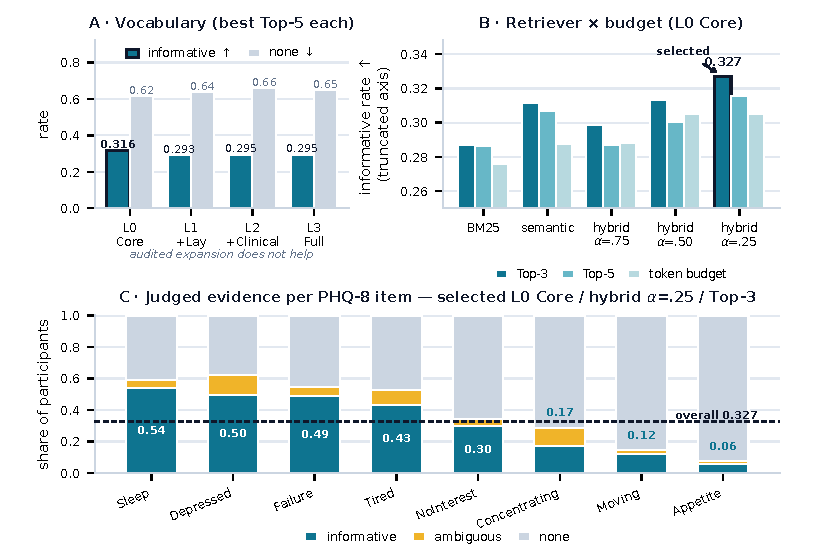
\includegraphics[width=\textwidth]{final_report_fig2_retrieval_selection.pdf}
  \caption{Systematic, label-free retrieval selection; all quantities are judge statuses over set-level evidence, with no PHQ label used. \textbf{(A)}~Best Top-5 configuration for each vocabulary tier. \textbf{(B)}~Informative rate for each retriever and evidence budget under the Core vocabulary; the vertical axis is truncated to resolve the differences, and the selected cell is outlined. \textbf{(C)}~Composition of judged statuses per PHQ-8 item under the selected configuration, ordered by informative rate; the dashed line marks the 0.327 overall rate. Rates describe what the interviews contain and what the retriever selected, not symptom prevalence, and the judge is a model-based audit rather than clinician-validated annotation.}
  \label{fig:r2-retrieval}
\end{figure}

\subsection{Downstream Consequences of the Selected Retrieval}
\label{subsec:r2-downstream}
Table~\ref{tab:r2-policies} compares the encoder training policies and the LLM evidence policies, and Figure~\ref{fig:severity-tradeoff} places every one of them on the severe-recall/false-severe plane. The selected retrieval does not directly improve the status-quo encoder over frozen R0. R2 status quo reaches macro-F1 0.359, QWK 0.361, and MAE 0.686; paired participant bootstrap intervals versus R0 include zero for all reported metrics. Masking judged-none rows increases macro-F1 slightly but reduces QWK and significantly increases far-off error by 0.0177 (95\% CI [0.0006, 0.0342]).

Dropping judged-none training rows produces the highest raw encoder scores: macro-F1 0.406, QWK 0.416, class-3 F1 0.339, and severe recall 0.299. Relative to status quo, gains in macro-F1, QWK, class-3 F1, and severe recall have 95\% confidence intervals excluding zero. However, false-severe rate also rises significantly from 0.028 to 0.049. Moreover, the policy removes 4,264 of 7,008 fold-specific training rows (60.8\%) and approximately half of gold class-3 rows, with some item--fold cells losing nearly all usable examples. It therefore changes the training population rather than merely suppressing noisy evidence and fails the predefined false-severe constraint. The selected encoder is consequently status quo, not the raw-best drop policy.

The LLM does not benefit consistently from the new evidence. Keeping R2 windows raises severe recall relative to frozen R0 Qwen but significantly worsens MAE and false-severe rate. Filtering \texttt{none} or placing informative windows first further increases severe sensitivity, but significantly degrades Macro-F1, MAE, far-off error, and false-severe behavior. Transcript fallback provides the best constraint-passing R2 condition, at QWK 0.405 and MAE 0.664, but does not surpass frozen R0 Qwen. Using long context for every item is worse than retrieved evidence and significantly reduces severe recall.

\begin{table}[tb]
  \caption{Encoder training policies and LLM evidence policies on the selected Core/hybrid-.25/Top-3 retrieval. A dagger marks a raw-best policy rejected by the safety and data-retention constraints; bold marks the selected condition within each model family.}
  \label{tab:r2-policies}
  \centering
  \scriptsize
  \adjustbox{max width=\textwidth}{%
  \begin{tabular}{lllrrrrrr}
    \toprule
    Family & Condition & Selected & Macro-F1 $\uparrow$ & QWK $\uparrow$ & MAE $\downarrow$ & F1$_3$ $\uparrow$ & Recall$_3$ $\uparrow$ & False-severe $\downarrow$ \\
    \midrule
    Encoder & \best{Status quo} & \best{yes} & 0.3590 & 0.3614 & 0.6861 & 0.2119 & 0.1497 & 0.0278 \\
    Encoder & Mask none & no & 0.3677 & 0.3587 & 0.6792 & 0.2026 & 0.1377 & 0.0233 \\
    Encoder & Drop none$^{\dagger}$ & no & \best{0.4063} & \best{0.4162} & \best{0.6701} & \best{0.3390} & \best{0.2994} & 0.0492 \\
    \midrule
    LLM & Frozen R0 tolerant SC & reference & \best{0.4000} & \best{0.4063} & \best{0.6410} & 0.2537 & 0.2036 & 0.0423 \\
    LLM & Keep R2 windows & no & 0.3849 & 0.3978 & 0.6866 & \best{0.2876} & 0.2575 & 0.0562 \\
    LLM & Filter none & no & 0.3480 & 0.3430 & 0.7631 & 0.2754 & \best{0.2754} & 0.0763 \\
    LLM & Informative first & no & 0.3518 & 0.3531 & 0.7631 & 0.2624 & 0.2695 & 0.0826 \\
    LLM & \best{Transcript fallback} & \best{yes} & 0.3838 & 0.4047 & 0.6644 & 0.2724 & 0.2275 & 0.0467 \\
    LLM & Long context & no & 0.3528 & 0.3824 & 0.7414 & 0.1991 & 0.1317 & \best{0.0202} \\
    \bottomrule
  \end{tabular}%
  }
\end{table}

\subsection{Complementarity, Cascades, and Final Recommendation}
\label{subsec:final-results}
Complementarity remains visible under the selected retrieval. Across all 1,752 examples, both selected components are correct on 26.1\%, only the encoder on 20.0\%, only the LLM on 22.4\%, and neither on 31.4\%. The LLM is uniquely correct more often for NoInterest, Appetite, Failure, Concentrating, and Tired; the encoder is uniquely correct more often for Depressed, Moving, and slightly for Sleep. Complementarity is weakest where it matters most: among 167 severe examples, both models are correct on only 5.4\%, only the encoder on 9.6\%, only the LLM on 17.4\%, and both are wrong on 67.7\%.

The leakage-safe cascades reduce ordinal error but do not meet the acceptance criterion, as Table~\ref{tab:final} shows. The LLM-first cascade obtains macro-F1 0.398, QWK 0.406, and MAE 0.626. Relative to the selected LLM, MAE and far-off error improve significantly, and false-severe rate falls from 0.047 to 0.024; however, severe recall also falls significantly from 0.228 to 0.180, while the QWK increase is not statistically established. The encoder-first cascade shows the same pattern more strongly. Neither new cascade surpasses the frozen Attention-MIL merged cascade, which remains the recommended final system. As Figure~\ref{fig:severity-tradeoff} makes visual, no configuration reaches the preferred upper-left region of high severe recall and low false-severe rate; this joint unreachability, rather than any single metric, is the study's central negative result.

\begin{table}[tb]
  \caption{Selected R2 components, leakage-safe cascades, and the frozen project-best system. New cascades are evaluated against the better selected component and use routing parameters fitted inside training folds.}
  \label{tab:final}
  \centering
  \scriptsize
  \adjustbox{max width=\textwidth}{%
  \begin{tabular}{lrrrrrr}
    \toprule
    Model & Macro-F1 $\uparrow$ & QWK $\uparrow$ & MAE $\downarrow$ & F1$_3$ $\uparrow$ & Recall$_3$ $\uparrow$ & False-severe $\downarrow$ \\
    \midrule
    Selected R2 encoder & 0.3590 & 0.3614 & 0.6861 & 0.2119 & 0.1497 & 0.0278 \\
    Selected R2 LLM & 0.3838 & 0.4047 & 0.6644 & 0.2724 & 0.2275 & 0.0467 \\
    R2 encoder-first cascade & 0.3806 & 0.3935 & 0.6473 & 0.2387 & 0.1737 & 0.0297 \\
    R2 LLM-first cascade & 0.3982 & 0.4062 & 0.6256 & 0.2553 & 0.1796 & 0.0240 \\
    \best{Frozen R0 Attention-MIL merged cascade} & \best{0.4090} & \best{0.4470} & \best{0.6060} & \best{0.2560} & 0.1980 & 0.0366 \\
    \bottomrule
  \end{tabular}%
  }
\end{table}

\begin{figure}[tbp]
  \centering
  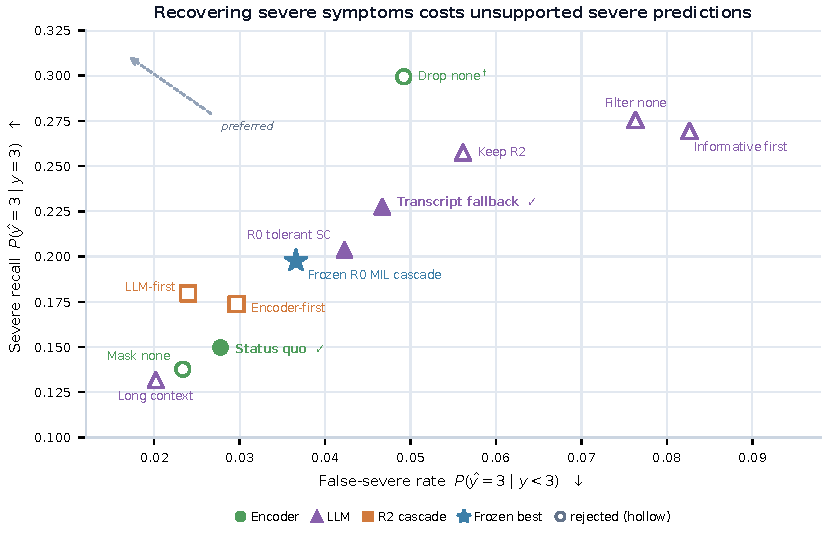
\includegraphics[width=\textwidth]{final_report_fig3_severity_tradeoff.pdf}
  \caption{Severe-sensitivity versus false-severe trade-off for every candidate system, on participant-grouped out-of-fold predictions ($n=1{,}752$, of which 167 are gold class-3). Marker shape encodes the model family; hollow markers denote configurations rejected by the predefined error and severe-class constraints, and a check mark denotes the condition selected within each family. Policies that recover more class-3 examples generally move right as well as up, so no system reaches the preferred upper-left region. Both error directions are consequential, and none of these operating points has been clinically validated.}
  \label{fig:severity-tradeoff}
\end{figure}

\subsection{Item-Level Failure Modes}
\label{subsec:item-results}
Evidence availability differs sharply by item under the selected retrieval, as Figure~\ref{fig:r2-retrieval}C shows. Sleep and Depressed have the highest informative rates, 0.539 and 0.498, followed by Failure (0.489) and Tired (0.434). NoInterest remains moderate at 0.301, whereas Concentrating (0.174), Moving (0.123), and especially Appetite (0.059) are usually judged \texttt{none}. These values describe the evidence selected from interviews, not symptom prevalence.

The language of each item helps explain the heterogeneity. Depressed mood and sleep changes are often expressed directly. NoInterest is frequently indirect, appearing as reduced activity or withdrawal rather than the literal item wording. Moving concerns psychomotor agitation or retardation, for which timing, voice, and visual behavior may be more informative than transcript words. Appetite is sparse in this interview protocol despite being linguistically concrete. The complementarity analysis also shows item-specific model roles: the LLM is uniquely correct most often for NoInterest and Appetite, while the encoder has a clearer advantage for Depressed and Moving. No single inference mechanism dominates all eight symptoms.

\section{Discussion}
\label{sec:discussion}
The study supports a three-part view of item-level depression prediction: evidence must be selected, severity must be inferred, and uncertainty must be converted into a safe model-selection decision. The components are coupled, but improvements are not interchangeable. The initial encoder is stable yet severe-blind; the LLM is more willing to call severe symptoms but produces more large and false-severe errors. A cascade helps only when its routing rule captures this complementarity without discarding the severe sensitivity that motivated the LLM.

The systematic retrieval experiment clarifies what improved evidence selection means in this setting. First, adding Lay and Clinical vocabulary does not improve judged evidence. The benefit comes instead from representing item meaning as coherent natural-language queries. Second, BM25 and semantic retrieval are complementary at the example level, but the optimal fusion is semantic-dominant: 75\% semantic and 25\% BM25. Third, Top-3 outperforms Top-5 and the encoder token budget, showing that evidence precision is more important than context volume. These findings argue against treating lexicon size or retrieved-token count as retrieval objectives.

Nevertheless, the better judged retrieval does not improve the final predictor. This mismatch has several possible explanations supported by the diagnostics. A set may be judged relevant without explicitly expressing PHQ frequency; retrieval can therefore improve topicality without resolving severity. Conversely, questionnaire labels may describe experiences not discussed in the interview. The very high \texttt{none} rate---60.8\% for the final R2 sets---indicates that missing transcript evidence is not a corner case. The improvement from \texttt{drop none} is consistent with label--evidence mismatch, but it is not a safe resolution: the policy removes most training rows, disproportionately changes severe examples, and significantly increases false-severe prediction.

The LLM evidence-policy results reinforce the same point. Removing judged-none windows does not simply remove noise. It can produce short, one-sided contexts that encourage over-calling, while long context can dilute item evidence and become too conservative. Transcript fallback offers a reasonable compromise but still does not outperform the frozen LLM. Thus, the evidence judge is useful for auditing and policy analysis, but its categories should not be treated as a complete training target or a substitute for human evidence annotation.

\subsection{Limitations and Clinical Interpretation}
The study uses 219 participants from one corpus and internal participant-grouped OOF analysis, not an external clinical cohort. Class 3 contains only 167 participant--item examples. The evidence judge has not been validated against a clinician-annotated evidence set and shares the Qwen family with the LLM predictor, creating possible circularity. The final Attention-MIL correction branch was not retrained on R2, so the comparison with the frozen best system mixes retrieval and encoder architecture. Speaker roles are not uniformly reliable, and text-only input omits acoustic and visual cues, particularly for psychomotor behavior. Long-context input is a model-specific truncated representation rather than an oracle view of the full interview. Retrieved excerpts are candidate evidence, not causal explanations, and reconstructed totals or threshold analyses are internal diagnostics rather than clinical validation. Both missed severe symptoms and unsupported severe predictions are consequential; any practical use would require human review, privacy safeguards, calibrated uncertainty, and external validation.

\section{Conclusion}
\label{sec:conclusion}
We formulated PHQ-8 item prediction from mental-health interviews as an evidence-conditioned ordinal task. A MentalBERT+CORN encoder provides ordinal safety but under-detects severe symptoms, whereas Qwen reasoning improves severe sensitivity at the cost of larger and false-severe errors. Their complementary failures support selective correction, and the frozen Attention-MIL merged cascade remains the strongest complete system at macro-F1 0.409, QWK 0.447, and MAE 0.606.

The systematic retrieval experiment yields a different kind of contribution. Audited vocabulary expansion does not help; natural-language multi-query retrieval does. BM25 and semantic search are complementary, but the selected evidence selector is semantic-dominant, using the Core vocabulary, 25\% BM25, 75\% semantic similarity, and three windows. This improves judged evidence quality but not final prediction. Aggressive missing-evidence policies expose a real label--transcript mismatch while creating unacceptable data-retention and false-severe trade-offs, and the new leakage-safe cascades do not surpass the frozen best system. Progress therefore requires not only better retrieval, but evidence annotations and routing objectives that jointly account for relevance, frequency, missing information, and safety.

\section*{Ethics and Broader Impact}
This work analyzes sensitive mental-health interviews and predicts symptom severities; it is research on model behavior, not a diagnostic instrument. Both error directions are consequential: missed severe symptoms may delay attention, while unsupported severe predictions may stigmatize or trigger unwarranted intervention. Retrieved excerpts must not be presented as validated clinical rationales. Any downstream use would require clinician oversight, consent-respecting data handling, uncertainty communication, and protection against disclosure of interview text. We do not redistribute E-DAIC transcripts or participant-linked generations.

\section*{Data and Code Availability}
E-DAIC is available from USC ICT under its license agreement. The project repository contains code, run scripts, aggregate metrics, selection artifacts, and non-sensitive result reports used in this paper. Transcript-bearing windows, raw generations, and licensed labels are not redistributed. Derived aggregate artifacts are sufficient to audit the reported comparisons, while access to the original corpus is required for full end-to-end reproduction.

\bibliographystyle{unsrt}
\bibliography{references_V9}

\end{document}
